\section{Иерархическое обучение с подкреплением}

\subsection{Опции}

Представьте, что ваша задача --- приготовить суп. Пытаться решить задачу методом проб и ошибок вам не придётся: у вас есть рецепт. Однако, беда: в рецепте первым пунктом написано <<возьмите чистую кастрюлю>>... И учиться брать чистую кастрюлю, видимо, придётся методом проб и ошибок.

Большинство задач в сложных средах делятся на подзадачи. <<Рецепта>>, позволяющего разложить сложную задачу на простые, однако, в общем случае нет, и агенту нужно не просто научиться решать набор подзадач, но и определять, какие именно подзадачи требуется выполнить для успеха.

Мы можем не вводить понятие подзадач или иерархичности и пытаться оптимизировать суммарную награду напрямую, как делали до этого. Но тогда наш рецепт для приготовления супа будет выглядеть примерно так: <<сожмите вот этот перечень мышц, теперь вот этот, так-так-так, ваша рука начала подниматься...>>. Введение иерархий позволит агенту смотреть на задачу на более абстрактном уровне --- на уровне выбора подзадач. Важно, что на этом уровне будет совершенно другой <<масштаб времени>>: число последовательных решений для решения всей задачи существенно сократится. Такое свойство <<высокоуровневых стратегий>> называется \emph{temporal abstraction}. Концептуально, именно на этом уровне агент должен заботиться о награде, описывающей основную задачу. Пока что, для начала, мы ограничимся чуть менее амбициозной задачей: давайте как-нибудь сделаем нашу стратегию <<многоуровневой>>, например, следующим образом.

\begin{definition}
\setcounter{footnote}{1}
Для данного MDP \emph{опцией} (\ENGLISH{option}) $g$ называется пара\footnote{в оригинале дополнительно рассматривалось множество $I_g \subseteq \St$ тех состояний, в которых опцию можно начать выполнять, однако в дальнейшем повествовании ситуация $I_g \ne \St$ нам не встретится.} $(\pi_g, \beta_g)$:
\begin{itemize}
    \item $\pi_g$ --- стратегия для исходного MDP.
    \item $\beta_g \colon \St \to [0, 1]$ --- \emph{политика терминальности} (termination policy).
\end{itemize}
\end{definition}

Пусть у нас есть множество опций $\G$, то есть даны или несколько разных стратегий $\pi_g$, или просто универсальная стратегия $\pi(a \mid s, g)$. Эти стратегии, работающие <<с исходным>> MDP на уровне \emph{примитивных действий} (primitive actions) (элементов $\A$), будем далее также называть \emph{рабочими} (workers). Также мы заводим <<высокоуровневую>> стратегию, которую далее будем называть \emph{менеджером} (manager) или \emph{мастер-стратегией} (master policy) $\manager{\pi}(g \mid s)$. Высокоуровневые действия также ещё называют \emph{макро-действиями}, а примитивные действия --- \emph{микро-действиями}.

На очередном шаге менеджер, исходя из текущего состояния $s_t$, выбирает опцию, которая будет далее работать в среде: $g_t \sim \manager{\pi}(g_t \mid s_t)$. Выбранный рабочий генерирует примитивное действие: $a_t \sim \pi(a_t \mid s_t, g_t)$. Среда переходит в новое состояние $s_{t+1} \sim p(s_{t+1} \mid s_t, a_t)$. И в этот момент вызывается политика терминальности опции $g$: с вероятностью $\beta_{t+1} \sim \mathrm{Bernoulli}(\beta_g(s_{t+1}))$ рабочий завершает свою работу и снова передаёт решение менеджеру (тот снова выбирает следующего рабочего, и так далее). Если же политика терминальности не срабатывает, менеджер не вызывается, и взаимодействовать со средой продолжает рабочий $\pi_{g_t}$.

Для удобства будем считать, что в рамках такого фреймворка в траекториях хранятся не только примитивные действия, но и решения менеджера вместе с решениями политики терминальности:
$$\Traj \coloneqq (g_0, a_0, r_0, s_1, \done_1, \beta_1, g_1, a_1, r_1, s_2, \done_2, \beta_2 \dots )$$
причём $g' = g$ с вероятностью 1, если $\beta' = 1$, и $\beta_0 = 0$. Таким образом, вероятностная модель порождения траекторий задана так:
$$\begin{cases}
g_t \sim \manager{\pi}(g_t \mid s_t) \quad & \text{если $\beta_t = 0$} \\
g_t = g_{t-1} \quad & \text{если $\beta_t = 1$} \\
\end{cases}$$
$$a_t \sim \pi(a_t \mid s_t, g_t)$$
$$s_{t+1} \sim p(s_{t+1} \mid s_t, a_t)$$
$$\beta_{t} \sim \mathrm{Bernoulli}(\beta_g(s_{t})) \quad (t > 0)$$

Мы поставим себе задачу обучать эту конструкцию end-to-end, то есть оптимизировать параметры стратегии менеджера, стратегий рабочих (опций) и политик терминальности опций напрямую с единственной целью максимизировать среднюю награду.

% \begin{theorem}
% Введение политики терминальности эквивалентно добавлению ещё одного элемента в пространство действий, выбор которого гарантирует завершение эпизода.
% \begin{proof}
% Пусть мы добавили ещё одно действие $a^+$ в $\A$ и задали стратегию рабочего следующим образом:
% \begin{align}\label{terminpolicyeq}
% \tilde{\pi}_g(a = a^+ \mid s) &\coloneqq \beta^g(s) \\
% \tilde{\pi}_g(a \ne a^+ \mid s) &\coloneqq (1 - \beta^g(s))\pi_g(a \mid s)
% \end{align}
% где $\pi_g$ --- исходная стратегия рабочего в исходной среде. Пусть среда также модифицирована так, что при выборе $a^+$ эпизод завершается. Тогда выбор действия эквивалентен использованию политики терминальности в исходной среде.
% \end{proof}
% \end{theorem}

\subsection{Semi-MDP}

Как нам это всё чудо обучать? Начнём с менеджера. Для простоты будем считать, что набор опций нам дан, то есть даны распределения $\pi_g(a \mid s)$ и $\beta_g(s)$; хотим научиться обучать $\manager{\pi}(g \mid s)$. Попробуем понять, не живёт ли он в каком-то MDP. Поскольку мы решили, что на вход он получает текущее состояние $\St$, то его пространство состояний такое же, как и в исходном MDP. Его пространством действий являются макро-действия $\G$. На каждом шаге менеджер выбирает $g \in \G$, после чего среда для менеджера работает так: стратегия-рабочий для выбранного $g$ бегает в настоящей среде и решает поставленную подзадачу, переводя среду в новое состояние $\manager{s}'$. То, в каком состоянии окажется среда по итогу, полностью задано вероятностной моделью --- для менеджера это можно рассматривать как функцию переходов $\manager{p}(\manager{s}' \mid s, g)$. Наконец, награда для менеджера за этот шаг есть сумма собранной за время работы рабочего награды основной цели:
\begin{equation}\label{managerreward}
\manager{r}(s, a) \coloneqq \sum_{t=0}^{\tau} \gamma^t r_t
\end{equation}
где $\tau$ --- число шагов, затраченных рабочим на решение задачи. И вот тут возникает нюанс.

Награду, который менеджер получит за второй шаг, необходимо дисконтировать на $\gamma^{\tau}$, поскольку в настоящем MDP прошло $\tau$ шагов. Более того, это $\tau$ --- случайная величина; рабочий мог потратить на решение как 10 шагов, так и 100. А значит, менеджер живём не совсем в MDP; для него действия имеют различную продолжительность по времени. Если раньше в MDP все действия, можно считать, гарантированно <<выполнялись>> один шаг, то теперь, для менеджера, это не так.

\begin{definition}
MDP называется \emph{полумарковским} (\ENGLISH{Semi-Markov decision process, sMDP}), если его функция перехода $p(s', \tau \mid s, a)$ помимо следующего состояния возвращает время $\tau > 0$, <<затраченное>> на выполнение данного шага. 
\end{definition}

В общем случае в sMDP время шагов может быть и вещественным числом (в частности, так можно учитывать, что среда взаимодействует с агентом в режиме <<реального времени>>), но в нашем случае $\tau > 0$ --- всегда натуральное число. Итак, при работе в sMDP в траекториях дополнительно необходимо хранить время каждого шага $\tau_t$; награда за $t$-ый шаг дисконтируется не на $\gamma^t$, а на $\gamma^{\sum_{t' \ge 0}^t \tau_{t'}}$.

Ранее рассматриваемая теория достаточно естественно обобщается на данный кейс. Например, уравнения Беллмана должны учитывать время в дисконтировании; например, для Q-функции:
$$Q^\pi(s, a) = r(s, a) + \E_{s', \tau} \gamma^\tau \E_{a'} Q^\pi(s', a')$$

Адаптация Q-learning для sMDP выглядит соответствующе: для перехода $(s, a, r, \tau, s', \done)$ обновление выглядит так:
$$Q^*(s, a) \leftarrow (1 - \alpha) Q^*(s, a) + \alpha \left(r + \gamma^\tau \max_{a'} Q^*(s', a') \right)$$
То есть по прошедшему времени $\tau$ мы тоже стохастически аппроксимируем: используем сэмпл из буфера вместе с сэмплом $s'$.

\subsection{Оценочная функция по прибытию (U-функция)}

Итак, менеджер живёт в полумарковском процессе принятия решений sMDP $(\St, \G, \manager{\Trans}, \manager{r})$, где $\manager{r}$ определено \eqref{managerreward}, а функция переходов $\manager{\Trans}$ задаётся процессом взаимодействия выбранного рабочего со средой с завершением по триггеру соответствующей политики терминальности. Мы, в принципе, можем полностью расписать это распределение $\manager{p}(\manager{s}', \tau \mid s, g)$, но это получится громоздко: нужно выинтегрировать $a_0, s_1, a_1, \dots s_{\tau - 1}, a_{\tau - 1}$, учесть вероятность попадания в $p(\manager{s}' \mid s_{\tau - 1}, a_{\tau - 1})$, срабатывание политики терминальности $\beta_g(\manager{s}')$ и несрабатывание политики терминальности для $s_1, s_2 \dots s_{\tau - 1}$ внутри интеграла.

Вместо этого удобнее работать с теорией на уровне одношаговых рекурсивных соотношений между величинами, где один шаг --- это генерация одной случайной величины. Раньше в обычных MDP мы как делали: сгенерировали действие, и вся будущая награда --- это Q-функция. Среда ответила нам сэмплом $s'$ (ещё наградой за шаг и флагом $\done$, но считаем, что это идёт <<в одном комплекте>>) --- и дальнейшая награда есть V-функция. Это было очень удобно, поскольку все эти оценочные функции легко выражались между собой. Нам надо поступить также для траектории, состоящей из случайных величин $g, a, s', \beta'$: выбор менеджера, выбор стратегии, отклик среды, выбор политики терминальности.

По определению, $\manager{Q}(s, g)$ обозначает следующее: менеджер сидел в некотором в состоянии $s$ и выбрал опцию $g$, или, что не существенно, опция $g$ уже была выбрана на предыдущем шаге, а политика терминальности не затриггерилась (в любом случае, в состоянии $s$ активировалась опция $g$), и функция возвращает среднюю будущую награду. Мы опустим здесь верхний индекс $\pi$, подразумевая, что мы считаем оценочную функцию для всего комплекта подконтрольных нам распределений: стратегии менеджера, рабочего и политик терминальности. Попробуем получить одношаговое рекурсивное соотношение для $\manager{Q}(s, g)$, связав её с оценочной функцией для следующей случайной величины --- выбором действия $a$ рабочим. Каким рабочим? Ну, раз активирована опция $g$, то однозначно рабочим $\pi(a \mid s, g)$. 

Мы уже поняли, что на стратегию рабочих можно смотреть как на универсальную стратегию в MDP с пространством состояний $\St \times \G$; однако выписать функцию переходов для них тоже довольно сложно, поскольку в ней замешаны функции терминальности и стратегия менеджера. Удобно смотреть на рабочих по-другому. При фиксированном менеджере и политике терминальности в их MDP с пространством состояний $\St \times \G$ и действиями $\A$ функция переходов устроена так: сэмплируется $s' \HM\sim p(s' \HM\mid s, a)$, и дальше с вероятностью $\beta(s', g)$ эпизод заканчивается, а за последний шаг агент получает награду $\manager{V}(s')$, иначе эпизод продолжается. Мы можем определить $V(s, g)$ и $Q(s, g, a)$ --- универсальные оценочные функции рабочих --- как оценочные функции в таком MDP, как будущие награды после реализации поступающих на вход случайных величин. Тогда в силу структуры вероятностной модели:
\begin{proposition}
$$\manager{Q}(s, g) = V(s, g) = \E_{\pi_g(a \mid s)} Q(s, a, g)$$
\end{proposition}

Попробуем пойти дальше и построить одношаговое соотношение для $Q(s, a, g)$. Тут нам для удобства понадобится ещё одна вспомогательная оценочная функция. Дело в том, что V-функция менеджера по определению предполагает, что первым следующем шагом генерации траектории будет сэмплирование действие менеджером --- $\manager{V}(s)$ есть хвост награды по траектории после попадания в $s$ при условии (!) срабатывания триггера $\beta \HM= 1$. Работать с этим неудобно, поскольку мы не знаем, сработал ли триггер или нет, и поэтому вводится вспомогательная U-функция --- это хвост награды по траектории после попадания в состояние $s$ без каких-либо дополнительных ограничений.

\begin{definition}
Для sMDP, заданного MDP с набором опций $\{\pi_g, \beta_g\}$, U-функцией или \emph{оценочной функцией по прибытию} (state-value function upon arrival) называется
% \begin{equation}\label{Ufunction}
% U^*(s', g) \coloneqq (1 - \beta^g(s'))\manager{Q}^*(s', g) + \beta^g(s') \max\limits_{g'} \manager{Q}^*(s', g')
% \end{equation}
\begin{equation}\label{Ufunction}
U(s', g) \coloneqq (1 - \beta^g(s'))\manager{Q}(s', g) + \beta^g(s') \manager{V}(s')
\end{equation}
\end{definition}

Что это за формула: на вход U-функция получает состояние, в которое <<входит>> агент, и текущую опцию. Дальше расписано мат.ожидание по срабатыванию триггера. Если политика терминальности не срабатывает, следующей опцией снова будет $g$, поэтому дальнейшяя награда эквивалентна $\manager{Q}(s', g)$. Иначе выбор переходит к менеджеру и мы получим $\manager{V}(s')$. Таким образом, по определению:

\begin{proposition}
\begin{equation}\label{QU}
Q(s, g, a) = r(s, a) + \gamma \E_{s'} U(s', g)
\end{equation}
\end{proposition}

% \begin{theorem}
% Функция переходов для менеджера задаётся следующим распределением:
% $$\manager{p}(\manager{s}', \tau = 1 \mid s, g) = \beta^g(\manager{s}')\int\limits_{\A} \pi_g(a \mid s)p(\manager{s}' \mid s, a) \diff a$$
% Для $\tau > 1$ справедлива рекуррентная запись:
% \begin{equation}\label{managertransrecur}
% \manager{p}(\manager{s}', \tau \mid s, g) = \int\limits_{\A}\int\limits_{\St} \pi_g(a \mid s)p(s' \mid s, a)(1 - \beta^g(s'))\manager{p}(\manager{s}', \tau - 1 \mid s', g) \diff a \diff s'
% \end{equation}
% \begin{proof}
% Первое утверждение следует из определений: для того, чтобы $\tau$ было равно 1, необходимо, чтобы рабочий управился за один шаг; для этого по действию рабочего проводится маргинализация.

% Второе утверждение следует из вероятностной модели: маргинализация проводится по первому действию и состоянию $s'$ среды после первого шага. Поскольку $\tau > 1$, то рабочий не должен был прекратить в $s'$ выполнение задачи, отсюда домножение на $1 - \beta^g(s')$ (рабочий не мог выбрать в $s'$ действие $a^+$). Наконец, после этого в силу стационарности $p(s' \mid s, a)$, $\pi_g(a \mid s)$ и $\beta^g(s)$ вероятность за $\tau - 1$ попасть из $s'$ в $\manager{s}'$ в точности равна $\manager{p}(\manager{s}', \tau - 1 \mid s', g)$.
% \end{proof}
% \end{theorem}

\subsection{Intra-option обучение}

Термин <<\emph{intra-option}>> означает, что мы можем за счёт таких соотношений обучать функции менеджера, используя информацию после выполнения каждого микро-действия (после получения информации о $s'$) вне зависимости от того, запускалась ли на данном шаге в принципе стратегия-менеджер или нет. Интуитивно основное соображение выглядит так: если стратегия-рабочий сделала один шаг в среде, а политика терминальности не сработала, то это всё равно что в этот момент менеджер снова выбрал того же самого рабочего.

Допустим, мы хотим обучить $\manager{Q}^*(s, g)$ менеджера в предположении, что политика терминальности и стратегии рабочего зафиксированы и не меняются. Тогда как будет выглядеть уравнение <<оптимальности>>?

\begin{definition}
Для sMDP, заданного MDP с фиксированным набором опций $\{\pi_g, \beta_g\}$, \emph{оптимальной U-функцией} называется
\begin{equation}\label{U*function}
U^*(s', g) \coloneqq (1 - \beta^g(s'))\manager{Q}^*(s', g) + \beta^g(s') \max\limits_{g'} \manager{Q}^*(s', g')
\end{equation}
\end{definition}

В этом определении мы по сути просто взяли обычной U-функции \eqref{Ufunction} и заменили в нём $\manager{V}^*(s')$ на $\max\limits_{g'} \manager{Q}^*(s', g')$ в силу оптимальности менеджера. Давайте теперь попробуем выразить $\manager{Q}^*(s, g)$ через неё же саму, используя $U^*(s', g)$.

\begin{proposition}\label{pr:managerQ*U*}
Q-функция менеджера удовлетворяет следующему рекурсивному уравнению:
\begin{equation}\label{managerQ*U*}
\manager{Q}^*(s, g) = \E_{\pi_g(a \mid s)} \left[ r(s, a) + \gamma \E_{s'} U^*(s', g)\right]
\end{equation}
\begin{proof}
Допустим, менеджер выбрал опцию $g$, и рабочий сделал один шаг в среде (сгенерировалось $a \sim \pi_g(a \mid s)$ и $s'$ в исходном MDP). Дисконтирование случилось только на $\gamma$. После этого с вероятностью $\beta^g(s')$ менеджер сможет выбрать новую подзадачу (это бы соответствовало обычному уравнению оптимальности Беллмана, поскольку прошёл всего один шаг), а с вероятностью $1 - \beta^g(s)$ менеджеру не предоставляется выбора. В такой ситуации можно считать, что менеджер просто <<обязан>> снова выбрать $g$: вероятностная модель со следующего шага выглядит в точности также.
\end{proof}
\end{proposition}

Итак, мы можем для обучения менеджера пользоваться Q-learning-ом для sMDP: просить рабочего $g$ решить подзадачу, дождаться $\manager{s}', \tau$ и делать один шаг обновления. Но <<intra-option>> рекурсивное уравнение \eqref{managerQ*U*} показывает интересную альтернативу: для обучения функции ценности менеджера для перехода $\T \coloneqq (s, g, a, r, s', \done)$ можно рассчитать целевую переменную как
$$y(\T) \coloneqq r(s, a) + \gamma (1 - \done) U^*(s', g),$$
где U-функция вычисляется полностью по формуле \eqref{U*function} (мат.ожидание по Бернуливской $\beta$ можем взять явно), и далее, как обычно, минимизировать MSE:
$$\E_\T \left(y(\T) - \manager{Q}^*(s, g)\right)^2 \to \min_{\manager{Q}^*}$$
Заметим, что переходы мы можем брать любые, в том смысле, что не обязательно, чтобы $g$ было выбрано менеджером именно на данном шаге. Для корректного обучения мат.ожиданий нам требуется лишь, чтобы $a \HM\sim \pi_g(a \HM\mid s)$, $r \HM= r(s, a)$ и $s' \HM\sim p(s' \HM\mid s, a)$. Обратим внимание на первое условие: сейчас мы считаем опции зафиксированным (частью стационарной среды). Если стратегии рабочих меняются (а они будут меняться, так как будут обучаться), условие стационарности нарушается, и off-policy режим обучения мы, естественно, теряем. 

\subsection{Обучение стратегий рабочих}

\begin{proposition}
В предположении оптимальности менеджера оптимальная Q-функция рабочего удовлетворяет следующему уравнению:
$$Q^*(s, a, g) = \left[ r(s, a) + \gamma \E_{s'} U^*(s', g)\right]$$
\begin{proof}
Доказательство в точности повторяет теорему \ref{pr:managerQ*U*} за тем исключением, что действие $a$ уже подано оценочной функции на вход.
\end{proof}
\end{proposition}

Мораль отсюда простая: чтобы учить оценочные функции рабочего, мы можем использовать те же таргеты $y(\T)$. Только теперь их оценочная функция просто <<обусловлена>> дополнительно на действие $a$.
$$\E_\T \left(y(\T) - Q^*(s, g, a)\right)^2 \to \min_{Q^*}$$

Важный момент --- здесь можно применять hindsight-приём, который мы встречали в разделе \ref{subsec:hindsight}. Действительно, поскольку единственное, что теперь требуется от переходов --- $s' \HM\sim p(s' \HM\mid s, a)$, мы можем проделать переразметку имеющегося в опыте перехода $\T \coloneqq (s, g, a, r, s', \done)$ на $\hat{\T} \coloneqq (s, \hat{g}, a, r, s', \done)$ для любого $\hat{g}$. То есть: что было бы, если бы в состоянии $s$ мы пользовались бы опцией $\hat{g}$ и выбрали бы действие $a$? Тогда мы попали бы в состояние $s'$ и получили бы награду $r$. Другой информации для получения прецедента для обучения $Q^*(s, \hat{g}, a)$ нам и не нужно. Это значит, что для рабочих мы можем обучать оценочные функции сразу для всех $g \in \G$.

Мы обсудили обучение Q-функций менеджера и рабочего с одношаговых таргетов; конечно же, имея на руках рекурсивные соотношения, мы можем построить полные аналоги всей стандартной теории. Например, для применения Policy Gradient подхода, нам нужны не сами оценочные функции, а их несмещённые оценки; в таких ситуациях достаточно иметь лишь достаточно обучать лишь Q-функцию менеджера. Действительно: если мы знаем $\manager{Q}(s, g)$, то тогда в силу \eqref{QU}:
$$Q(s, g, a) \approx r(s, a) + \gamma U(s', g), \quad s' \sim p(s' \mid s, a),$$
где $U(s', g)$ выражается через Q-функцию менеджера в силу формулы \eqref{Ufunction} --- несмещённая оценка. В качестве бэйзлайна возможно использовать $V(s, g)$, которая совпадает с $\manager{Q}(s, g)$.

\subsection{Обучение функций терминальности}

Перейдём к оставшемся открытому вопросу: как обучать политику терминальности? Рассмотрим такую ситуацию: мы сидим в состоянии $s$ и выполняем опцию $g$. Нужно ли останавливать рабочего, полагая $\beta(s, g) \HM= 1$, или можно продолжать действовать с его помощью? С точки зрения оптимальных оценочных функций, в первом случае мы получим $\manager{V}^*(s)$, а во втором $V^*(s, g)$. Но очевидно, что
$$\manager{V}^*(s) = \max_{\hat{g}} \manager{Q}^*(s, \hat{g}) \ge \manager{Q}^*(s, g) = V^*(s, g),$$
то есть оптимально прерывать рабочего на каждом шаге.

Это, конечно, затыка в нашей теории, поскольку если рабочий прерывается на каждом шаге, никакого temporal abstraction у нас не получится. Попробуем обратится к Policy gradient подходу; мы сможем обучать функции терминальности, пользуясь формулой градиентов по их параметрам, когда сами политики терминальности будут стохастичны. 

Пусть $\beta(s, g, \theta) \in [0, 1]$ выдаёт вероятность бернулливской величины и дифференцируемо по параметрам $\theta$. Пусть $\manager{A}(s, g) \coloneqq \manager{Q}(s, g) \HM- \manager{V}(s)$ --- Advantage-функция менеджера. Функционал, который мы оптимизируем, для начального состояния $s_0$, равен по определению $\manager{V}(s_0)$.

\begin{theorem}[Termination Gradient Theorem]
\begin{equation}\label{terminationpg}
\nabla_{\theta} \manager{V}(s) = -\E_{\Traj \mid s_0 = s} \sum_{t \ge 0} \gamma^t \nabla_\theta \beta(s_t, g_t, \theta) \manager{A}(s_t, g_t)
\end{equation}
\begin{proof}
По определению:
$$\nabla_{\theta} \manager{V}(s) = \nabla_{\theta} \E_{g} \E_{a} \left[ r(s, a) + \gamma \E_{s'} U(s', g)\right]$$
Мат.ожидания здесь берутся по стратегиям менеджера и рабочего, не зависящих от $\theta$, поэтому мы сразу проносим градиент вплоть до оценочной функции по прибытию, а дальше применяем стандартную для Policy Gradient технику.
\begin{align*}
\nabla_{\theta} U(s', g) &= \nabla_{\theta} \left[\beta(s', g, \theta) \manager{V}(s') + (1 - \beta(s', g, \theta)) \manager{Q}(s', g) \right] = \\
 &= \nabla_{\theta} \beta(s', g, \theta) \left[\manager{V}(s') - \manager{Q}(s', g) \right] + \beta(s', g, \theta) \nabla_{\theta} \manager{V}(s') + (1 - \beta(s', g, \theta)) \nabla_{\theta} \manager{Q}(s', g)
\end{align*}
Здесь мы хотим вернуться к мат.ожиданиям по траекториям, и в том числе к мат.ожиданиям по $\beta$. Для этого достаточно заметить, что в полученном выражении ровно такое мат.ожидание и стоит. Действительно, убедимся, что
$$\beta(s', g, \theta) \nabla_{\theta} \manager{V}(s') + (1 - \beta(s', g, \theta)) \nabla_{\theta} \manager{Q}(s', g) = \E_{\beta} \E_{g'} \nabla_{\theta} \manager{Q}(s', g')$$
Если в выражении справа выпало $\beta = 0$, то дальше гарантировано $g' = g$, мат.ожидание по $g'$ вырождается и мы получаем второе слагаемое из выражения слева. Если же в выражении справа выпало $\beta = 1$, то дальше $\E_{g'} \nabla_{\theta} \manager{Q}(s', g') = \nabla_{\theta} \manager{V}(s')$, и мы получаем первое слагаемое из выражения слева.

Собирая всё вместе, получаем рекурсивную формулу:
$$\nabla_{\theta} \manager{V}(s) = \E_{g} \E_{a} \gamma \E_{s'}  \left[ - \nabla_{\theta}\beta(s', g, \theta) \manager{A}(s', g) + \E_{\beta} \nabla_{\theta} \manager{Q}(s', g') \right] $$
Собирая рекурсивную формулу в мат.ожидание по всей траектории, получаем доказываемое.
\end{proof}
\end{theorem}

Крайне интуитивная формула \eqref{terminationpg} говорит ровно то, с чего мы начали обсуждение оптимального поведения политики терминальности: если $\manager{A}(s, g) \HM> 0$, то текущая опция лучше той, которую в среднем выбрал бы текущий менеджер, и поэтому стоит продолжать её выполнять; $\beta(s, g)$ уменьшается. Но если $\manager{A}(s, g) < 0$, то менеджер сейчас может выбрать более хорошую опцию, более хорошего рабочего, и поэтому нужно передавать ему управление: $\beta(s, g)$ надо уменьшать.

Как мы знаем, для оптимальных стратегий $\max\limits_{g} \manager{A}(s, g) = 0$, и поэтому такая градиентная оптимизация чревата вырождающими ситуациями. Типично, что менеджер начнёт получать управление на каждом шаге. Бороться с этим приходится костылями: например, дополнительными регуляризациями на политику терминальности, чтобы она как можно реже передавала управление менеджеру, и менеджеры с рабочим учились в этих условиях с <<неоптимальной>> политикой терминальности. Популярное решение --- добавить в формуле \eqref{terminationpg} к оценке Advantage небольшое положительное число.

\subsection{Option-Critic}

Соберём всё вместе в алгоритм Option-Critic\footnote{ряд деталей этой сборки остаётся под вопросом. В частности, странно, что в policy gradient алгоритме используются одношаговые оценки.}. Итак, заводим нейросеть, принимающую на вход $s$, и имеющую следующие головы: оценочную функцию $\manager{Q}(s, g)$ для $g \in \G$, где $|\G|$ --- конечно (например, 4 или 8), $|\G|$ стратегий рабочих $\pi(a \mid s, g)$, а также $|\G|$ функций терминальности $\beta(s, g) \in [0, 1]$. Для обучения критика пользуемся intra-option обучением; для остальных голов используем формулы градиентов. В качестве стратегии менеджера будем использовать $\eps$-жадную стратегию на основе выученной $\manager{Q}(s, g)$.

\begin{algorithm}{Option-Critic}
\textbf{Гиперпараметры:} $M$ --- количество параллельных сред, $N$ --- длина роллаутов, $|\G|$ --- число рабочих, $\manager{Q}$ --- нейросеть с параметрами $\theta$, $\pi$ --- нейросеть универсальной стратегии рабочих, $\beta$ --- нейросеть для политики терминальности, SGD оптимизатор.

\vspace{0.3cm}
Инициализировать $\theta$ \\
\textbf{На каждом шаге:}
\begin{enumerate}
    \item в каждой параллельной среде собрать роллаут длины $N$, используя иерархическую стратегию с менеджером $\eps\operatorname{-greedy}(\manager{Q}(s, g))$ и опциями $\beta, \pi$:
    $$s_0, g_0, a_0, r_0, s_1, g_1 \dots , s_N$$
    \item для каждой пары $s, g$ из каждого роллаута посчитать оценки $\manager{V}, \manager{A}$, игнорируя зависимость оценки от параметров $\theta$:
    $$\manager{V}(s) \coloneqq \sum_{\hat{g}} \manager{\pi}(\hat{g} \mid s) \manager{Q}(s, \hat{g})$$
    $$\manager{A}(s, g) \coloneqq \manager{Q}(s, g) - \manager{V}(s)$$
    \item для каждой пары $g, s'$ из каждого роллаута посчитать ценность по прибытию, игнорируя зависимость оценки от параметров $\theta$:
    $$U(s', g) \coloneqq (1 - \beta(s', g)) \manager{Q}(s', g) + \beta(s', g) \manager{V}(s')$$
    \item для каждого перехода $\T \coloneqq (s, g, a, r, s', \done)$ посчитать таргет для критика:
    $$y(\T) \coloneqq r + \gamma (1 - \done) U(s', g)$$
    \item вычислить лосс критика:
    $$\Loss^{\critic}(\theta) \coloneqq \frac{1}{MN}\sum_{\T} \left( y(\T) - \manager{Q}(s, g) \right) ^2$$
    % \item вычислить градиент для менеджера:
    % $$\nabla^{\mathrm{manager}}_\theta \coloneqq \frac{1}{MN}\sum_{\T} \nabla_\theta \log \manager{\pi}_\theta(g \mid s) \left( \manager{Q}(s, g) - \manager{V}(s) \right) $$
    \item вычислить градиент для рабочих:
    $$\nabla^{\mathrm{worker}}_\theta \coloneqq \frac{1}{MN}\sum_{\T} \nabla_\theta \log \pi_\theta(a \mid s, g) \left( y(\T) - \manager{Q}(s, g) \right) $$
    \item вычислить градиент для политик терминальности:
    $$\nabla^{\mathrm{termination}}_\theta \coloneqq -\frac{1}{MN}\sum_{\T} \nabla_\theta \beta(s, g) \manager{A}(s, g) $$
    \item сделать шаг градиентного спуска по градиенту $-\nabla^{\mathrm{worker}}_\theta - \nabla^{\mathrm{termination}}_\theta + \nabla_\theta \Loss^{\critic}(\theta)$
\end{enumerate}
\end{algorithm}

\subsection{Феодальный RL}

В рамках Option-Critic подхода мы не факт, что выучим какие-то разумные подзадачи; скорее, мы надеемся, что, возможно, рабочие как-то <<распределят>> между собой области среды, за которые будут ответственны. Мы понимаем, что, деля сложную задачу на последовательность более мелких, мы можем переставать думать об исходной задаче не уровне выполнения подзадач. 

\begin{example}
То есть: если было принято решение достать чистую кастрюлю, то истинную цель этой установки (награду за приготовление супа) можно не принимать в расчёты и оптимизировать только награду за доставание кастрюли. Такое мышление открывает возможности для переиспользования оптимальных стратегий доставания кастрюли для других задач (например, приготовления пельменей) --- потенциальный путь к transfer learning.
\end{example}

Соображение лежит в основе принципа \emph{феодализма} (feudalism), который можно сформулировать в виде следующих постулатов:
\begin{itemize}
    \item стратегия, действующая на некотором уровне абстрактности, не должна задумываться о более высокоуровневых задачах (<<единственная задача вассала --- выполнение задач, поставленных феодалом>>).
    \item высокоуровневая стратегия не рассматривает примитивные действия $\A$ (<<феодала не заботит, как вассал будет достигать поставленных ему целей>>).
    \item при наличии нескольких уровней иерархии действует принцип <<вассал моего вассала не мой вассал>>. В дальнейшем повествовании мы ограничимся двумя уровнями иерархии, но теорию легко можно обобщить на большее число уровней.
\end{itemize}

В общем случае, для каждого макро-действия $g$ задана своя стратегия рабочего $\pi_g$, однако мы можем пользоваться нотацией multi-task RL и использовать универсальные стратегии и оценочные функции, принимающие на вход пару $s, g$.

Итак, общая схема иерархического RL с двумя уровнями, к которой мы хотим прийти, выглядит так. Откуда-то берётся набор подзадач; необходимо придумать, откуда его брать. Заводится стратегия-менеджер и стратегии-рабочие для каждой подзадачи. Когда менеджер выбирает подзадачу $g$, запускается стратегия соответствующего рабочего $\pi_g$. Она делает несколько шагов в исходной среде, пока не решит задачу или не <<сдастся>> (кастрюли в шкафу не оказалось и нужно бежать в магазин за новой); критерий остановки процесса выполнения стратегии рабочего остаётся открытым. Далее менеджер снова принимает решение о следующей решаемой подзадаче, оптимизируя исходную награду; рабочие стремятся решить свои подзадачи, для чего им нужно как-то задать функцию награды. 

\begin{example}
В идеале, иерархический RL должен выглядеть как-то примерно так. Менеджер смотрит на текущее состояние и говорит: нужно добраться до банка! Откуда-то берётся функция награды, описывающая задачу $g$ <<добраться до банка>>, и соответствующая стратегия рабочего $\pi(a \mid s, g)$ в течение многих шагов эту задачу решает. В банке происходит определение того, что задача решена, и управление снова передаётся менеджеру. Тот видит, что агент находится в банке, и выбирает новую задачу $g$, например, <<найти кучу денег>>. Вызывается новая стратегия рабочего, он снова решает задачу, менеджер выбирает следующую подзадачу, и так далее.

\begin{center}
    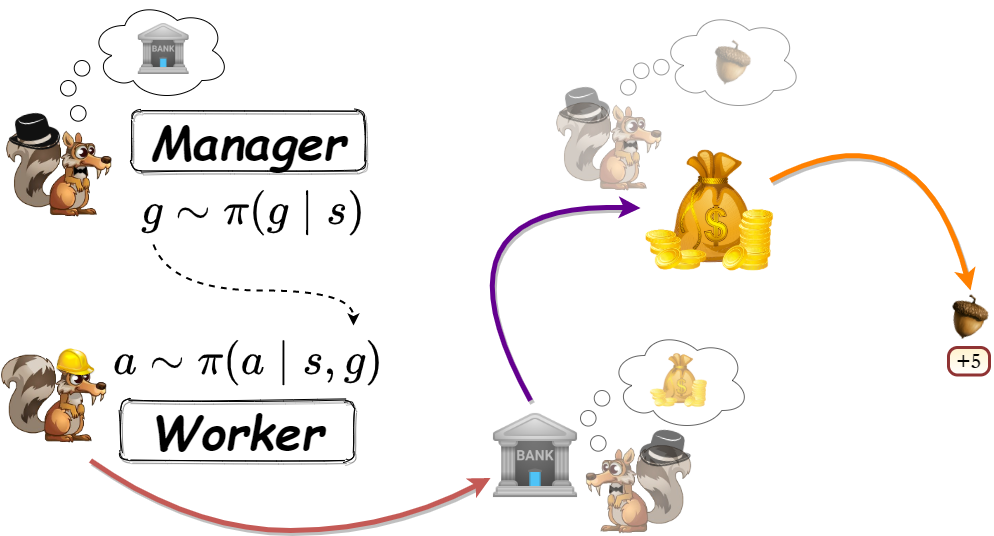
\includegraphics[width=0.8\textwidth]{Images/HRL4}
\end{center}
\end{example}

Иными словами, задачи и подзадачи в концепции RL всегда задаются MDP, и для подобных иерархических RL-алгоритмов нам нужно определиться, что есть MDP для той стратегии, которая принимает решение о подзадачах, и что есть MDP подзадач.

Строить такую идеальную схему, чтобы алгоритм сам смог выучить и набор подзадач, и механизмы определения моментов передачи управления менеджеру, мы на текущий момент не умеем. В Option-Critic мы абстрагировались от идей подзадач и оптимизировали всю нашу иерархическую конструкцию на максимизацию исходной функции награды, а основная сложность заключалась в обучении политики терминальности, и с ней же были связаны основные причины нестабильности процесса обучения. В рамках двух следующих алгоритмов мы будем следовать заветам феодального RL: выберем какой-нибудь набор подзадач, но упростим схему, убрав политику терминальности и заменив её на эвристики.

\subsection{Feudal Networks (FuN)}

Напрашивается в качестве набора подзадач брать задачу достижения некоторого состояния $g \in \St$. Основная идея \emph{феодальных сетей} (feudal networks) в том, чтобы задавать рабочим не целевое состояние, а направление, в котором нам хотелось бы сдвинуться, в пространстве латентных описаний состояний. Для этого менеджер переводит текущее состояние $s_t$ в латентное пространство $z_t \coloneqq f_\theta(s_t) \in \R^d$, где $\theta$ --- параметры, после чего генерирует вектор $g_t \in \R^d$. Выданный менеджером вектор нормируется, так что $\|g_t\|_2 = 1$: эта хитрость нужна, чтобы запрашиваемое направление не близко к тривиальному нулевому смещению и не достаточно <<большое>>.

Вместо политик терминальности вводится следующее упрощение: менеджер всё-таки будет вызываться на каждом шаге, и для каждого $s_t$ будет генерироваться целевое направление $g_t$; но обучаться он будет, исходя из предположения, что рабочий действительно выполняет поставленную задачу, и через $K$ шагов, где $K$ --- гиперпараметр, агент успешно сдвинется в указанном менеджером направлении. Иначе говоря, для функции переходов менеджера (которая составлена композицией настоящей функции перехода и стратегии рабочего) вводится следующее предположение:
$$\Prob (z_{t + K} = z_t + g_t) = 1$$
Здесь $z_{t+K} \coloneqq f_{\theta}(s_{t+K})$ --- латентное описание состояния через $K$ шагов. В жёсткой форме с подобной функцией переходов работать всё равно не столь удобно, поэтому вместо этого предположим более мягкую форму:
\begin{equation}\label{misesfishermanager}
    p(z_{t + K} \mid z_t, g_t) \propto \exp(d(z_{t+K} - z_t, g_t)),
\end{equation}
где $d$ --- некоторое расстояние между векторами, например, косинусное (с учётом того, что $\|g_t\|_2 = 1$):
$$d(z_{t+K} - z_t, g_t) = \frac{(z_{t+K} - z_t)^Tg_t}{\|z_{t + K} - z_t\|_2}$$
В таких предположениях нас волнует лишь направление $z_{t + K} - z_t$, в котором сдвинулось состояние; можно считать, что его мы тоже отнормировали, и тогда предположение \eqref{misesfishermanager} просто задаёт распределение на единичной сфере с центром в $z_k$, у которого мода находится в $g$, и чем менее скоррелированы выбранное направление и <<цель>> $g$, тем меньше вероятность.
\begin{definition}
Распределение 
\begin{equation}\label{misesfisher}
   p(d \mid g) \propto \exp(d^Tg),
\end{equation}
где $\|g\| \HM= 1$ и $\|d\| \HM= 1$, называется \emph{распределением Мизес-Фишера} (von Mises-Fisher distribution).
\end{definition}

%Прочитать про это распределение можно, например, \href{https://en.wikipedia.org/wiki/Von_Mises–Fisher_distribution}{здесь}.

\begin{proposition}
Нормировочная константа распределения Мизес-Фишера \eqref{misesfisher} не зависит от $g$
\begin{proof} Рассмотрим нормировочную константу для $g$:
$$\int\limits_{\|d\| = 1} \exp(d^Tg) \diff d$$
Возьмём какое-нибудь другое единичное направление $\hat{g}$. Сделаем замену переменных: пусть $M$ - матрица поворота, переводящая $\hat{g}$ в $g$: $g = M \hat{g}$. Тогда сделаем замену переменных: $\hat{d} \coloneqq M^T d$. Если $d$ пробегает единичную сферу, то так как $M$ --- матрица поворота, $\hat{d}$ тоже пробегает единичную сферу; определитель матрицы поворота $M$ также единичен, поэтому при замене переменной новых множителей не возникает. Получаем
$$\int\limits_{\|d\| = 1} \exp(d^TM\hat{g}) \diff d = \int\limits_{\|\hat{d}\| = 1} \exp(\hat{d}^T\hat{g}) \diff \hat{d},$$
что есть нормировочная константа для $\hat{g}$.
\end{proof}
\end{proposition}

Менеджер может считать, что, выбирая действие $g_t$, он выбирает состояние, в котором окажется через $K$ шагов, причём предлагается считать, что это распределение задано \eqref{misesfishermanager}, то есть:
$$\log \manager{\pi}(g_t \mid s_t) \coloneqq \log p(z_{t + c} \mid z_t, g_t) = d(z_{t+c} - z_t, g_t) + \const(\theta)$$

Подставляя это в формулу градиента для актёра, получается (для одного перехода) следующая формула:
$$\nabla_{\theta}^{\mathrm{manager}} = \nabla_{\theta} d(z_{t+K} - z_t, g_t(\theta)) \manager{A}^{\pi}(s_t, g_t)$$
Здесь $\manager{A}$ - Advantage-оценка критика менеджера (оцениваемая стандартным для Policy Gradient методов через обучение единственной функции $\manager{V}$), а зависимость $z_t, z_{t+K}, \manager{A}$ от параметров $\theta$ игнорируется.

% Для универсальной стратегии рабочего предлагается необычная архитектура сети. Предлагается не подавать рабочему указание менеджера $g_t$ на вход вместе с состоянием; вместо этого, актёр по текущему состоянию $s_t$ выдаёт матрицу ембеддингов действий $U_t \in \R^{|\A| \times d}$; берёт вектор усреднённых по последним $K$ шагам выданных менеджером направлений
% $$w_t \coloneqq \sum_{t' = t - K}^t g_t,$$
% и выдаёт в качестве стратегии над микродействиями
% $$\pi(a_t \mid s_t) \coloneqq \softmax{U_tWw_t},$$
% где $W \in \R^{d \times d}$ --- обучаемая матрица линейного преобразования указания $w_t$. Смысл подобной параметризации в том, чтобы гарантировать, что рабочий не игнорирует указания менеджера, и не возникало ситуации, что действия менеджера на результат не влияют, когда универсальная стратегия рабочего, игнорируя вход $g_t$, просто схлопывается к обычной, <<неиерархичной>>, стратегии.

Награда для рабочего в задаче следования тем направлениям, которые указывает менеджер, может быть сформулирована так:
$$r^{g}_t \coloneqq \frac{1}{K}\sum_{i = 0}^{K} d(z_t - z_{t - i}, g_{t - i}),$$
то есть для каждого из последних $K$ шагов проверяется, насколько точно рабочий следует указаниям менеджера, смещается ли в латентном пространстве менеджера описание состояния в указанном им направлении. Эта награда смешивается с наградой из исходного MDP; можно считать, что $r^{g}_t$ для рабочего --- внутренняя мотивация, а истинная награда из среды --- внешняя мотивация.

\subsection{HIRO}

Алгоритм HIRO в целом похож на FuN, хотя общая схема иерархической стратегии выглядит чуть-чуть по-другому. В этом алгоритме авторы рассматривали задачи непрерывного управления и могли для простоты положить $\G \equiv \St$, не переводя состояния в латентное пространства. Менеджер выбирает цель $g_t \in \St$ раз в $K$ шагов, где $K$ --- гиперпараметр. В последующие $K - 1$ моментов времени цели определяются по предыдущей по следующему <<векторному>> правилу:
$$g_{t + 1} - s_{t + 1} = g_t - s_t \qquad \Rightarrow \qquad g_{t + 1} = g_t + s_{t + 1} - s_t$$
Другими словами, если на шаге $t$ менеджер решил, что состояние $s_t$ должно меняться <<в направлении>> $g_t$, то дальше следующие $K$ шагов мы считаем, что хотим этому направлению следовать. Вызов раз в $K$ шагов кажется костылём, но позволяет избежать альтернативы с эвристикой FuN, в котором мы при обучении менеджера предполагали, что рабочий успешно выполняет возложенную на него задачу; тут же менеджера можно обучать лобовым подходом: он живёт даже не в sMDP, а обычном MDP, поскольку всегда гарантируется, что выбранное макро-действие будет выполняться в точности $K$ шагов. Однако, поскольку рабочие будут постепенно обучаться, это MDP нестационарное.

Внутренней мотивацией рабочего, выполняющего цель $g$, полагается расстояние от состояния, в которое попал агент, до целевого состояния $s_t + g_t$:
$$r^{\intr}(s_t, g_t, s_{t+1}) = -\|s_{t + 1} - (s_{t} + g_t)\|_2$$
Как и в FuN, такая внутренняя мотивация смешивается со внешней мотивацией --- наградой из основного MDP. 

Заметим, что рабочего можно спокойно обучать в off-policy режиме. Хотелось бы научиться обучать в off-policy режиме и менеджера, но понятно, что пространство действий $\G$ для менеджера с ходом обучения меняет своё семантическое значение. Предлагается лайфхак, очень похожий на идею переразметки траекторий из multi-task RL. Сохраним для менеджера в реплей буфера для $s_t, g_t$ всю последующую траекторию $a_t, s_{t+1} \dots a_{t + K - 1}, s_{t + K}$. Допустим, мы засэмплировали этот переход из буфера и хотим использовать для обучения. Проблема в том, что $\pi^g$ для $g$ из перехода уже может быть совершенно другим, и вероятность, что он сгенерировал бы такую траекторию, неприемлемо низкая. Идея: попробуем найти другое $\hat{g} \in \G$, для которого эта вероятность довольно высокая. То есть, мы приблизительно попытаемся решить следующую задачу:
$$\log p(a_t, s_{t+1} \dots a_{t + K - 1}, s_{t + K} \mid s_t, \hat{g}) \to \max_{\hat{g}}$$

Рассмотрим, из чего состоит правдоподобие. Мы предполагаем, что менеджер делает выбор в момент времени $t$, то есть менеджер больше на это правдоподобие не влияет. Есть логарифмы переходов $p(s' \mid s, a)$, которые не зависят от $\hat{g}$, поэтому их можно опустить. Остаются только правдоподобия выборов действий:
$$\sum_{t' = t}^{t + K - 1} \log \pi_{\hat{g}}(a_t \mid s_t) \to \max_{\hat{g}}$$

Почти всегда мы можем для данного $\hat{g}$ посчитать значение выражения. Предлагается взять несколько (штук восемь-десять) $g$, посчитать значение выражения и выбрать наилучшее. 

Какую хорошую стратегию перебора для сэмлпирования кандидатов $g$ выбрать? Поскольку агент в итоге сдвинулся на вектор $s_{t + K} - s_t$, то можно использовать этот вектор в качестве центра гауссианы, из которой будет проводиться сэмплирование. Также предлагается попробовать взять $g$ из буфера и сам центр $s_{t + K} - s_t$.